%!TEX TS-program = xelatex
\documentclass[10pt, compress]{beamer}

\usetheme[usetitleprogressbar]{m}

\usepackage[export]{adjustbox}
\usepackage{etoolbox}
\usepackage{booktabs}
\usepackage{dcolumn}
\usepackage[scale=2]{ccicons}
\usepackage{color}

% math typesetting
\usepackage{array}
\usepackage{amsmath}
\usepackage{amssymb}
\usepackage{amsthm}
\usepackage{amsfonts}
\usepackage{relsize}
\usepackage{mathtools}
\usepackage{bm}

% tables
\usepackage{tabularx}
\usepackage{booktabs}
\usepackage{multicol}
\usepackage{multirow}
\usepackage{colortbl}

% graphics stuff
\usepackage{subfig}
\usepackage{graphicx}
\usepackage[space]{grffile} % allows us to specify directories that have spaces
\usepackage{tikz}

% to change enumeration symbols begin{enumerate}[(a)]
\usepackage{enumerate}

% Add some colors
\definecolor{red1}{RGB}{253,219,199}
\definecolor{red2}{RGB}{244,165,130}
\definecolor{red3}{RGB}{178,24,43}

\definecolor{green1}{RGB}{229,245,224}
\definecolor{green2}{RGB}{161,217,155}
\definecolor{green3}{RGB}{49,163,84}

\definecolor{blue0}{RGB}{255,247,251}
\definecolor{blue1}{RGB}{222,235,247}
\definecolor{blue2}{RGB}{158,202,225}
\definecolor{blue3}{RGB}{49,130,189}
\definecolor{blue4}{RGB}{4,90,141}

\definecolor{purple1}{RGB}{191,211,230}
\definecolor{purple2}{RGB}{140,150,198}
\definecolor{purple3}{RGB}{140,107,177}

\definecolor{brown1}{RGB}{246,232,195}
\definecolor{brown2}{RGB}{223,194,125}
\definecolor{brown3}{RGB}{191,129,45}

% square bracket matrices
\let\bbordermatrix\bordermatrix
\patchcmd{\bbordermatrix}{8.75}{4.75}{}{}
\patchcmd{\bbordermatrix}{\left(}{\left[}{}{}
\patchcmd{\bbordermatrix}{\right)}{\right]}{}{}

% easy command for boldface math symbols
\newcommand{\mbs}[1]{\boldsymbol{#1}}

% command for R package font
\newcommand{\pkg}[1]{{\fontseries{b}\selectfont #1}}

% approx iid
\newcommand\simiid{\stackrel{\mathclap{\normalfont\mbox{\tiny{iid}}}}{\sim}}

% references to graphics
\makeatletter
%\def\input@path{{/Users/janus829/Research/netsMatter/prezzy/graphics/}, {/Users/s7m/Research/netsMatter/prezzy/graphics/}}
%\graphicspath{{/Users/janus829/Research/netsMatter/prezzy/graphics/}, {/Users/s7m/Research/netsMatter/prezzy/graphics/}}

\title[China]{\textsc{A Latent Space Approach to
Understanding Elite Coappearances in China}}
\author[Gallop et al.]{Max Gallop, Narisong Huhe, and Shahryar Minhas}

\date{\today}

\begin{document}
\frame{\titlepage}

%%%%%%%%%%%%%%%%%%%%%%%%%%%%%%%%%%%%%%%%%%%%%%%%%%%%%%%%%%%%
\frame{
  \frametitle{Motivation}

  % \vspace{-10mm}
Understanding elite networks and relationships is valuable:
  \begin{itemize}
    \item How they change over time.
    \item Relationship to political outcomes.
  \end{itemize}

  \centering
  \begin{tabular}{lr}
  \includegraphics[width=.5\textwidth]{XiLi} &  \includegraphics[width=.5\textwidth]{MittTrump} \\
  \end{tabular}
}
\frame{
  \frametitle{Motivation}

  \vspace{-10mm}
Elite politics in autocracies is:
  \begin{itemize}
    \item More important.
    \item More opaque.
  \end{itemize}
  We have limited information about elite relationships, but we have some information, notably for this paper we often have data on elites' public appearances.

}

\frame{
  \frametitle{Our Goal}

  \vspace{-10mm}
Leverage patterns of public appearances through a latent factor network to estimate factions in the Chinese Communist Party.

Evaluation Criterion:
  \begin{enumerate}
    \item Face validity: Relationships uncovered make sense to those with subject matter expertise.
    \item Predictive power: Use of our estimates improves performance of a downstream model of appointment to a key policymaking body.
  \end{enumerate}

}

\frame{
  \frametitle{Assumptions}
\begin{itemize}
\item Public events are strategic foci around which elites signal and manage their relationships.
\item These events reveal both relative prominence/position and relationships.
\item These events can best be conceived as relational data.
\end{itemize}

}

\frame{
  \frametitle{Three ``Who" Questions}
\begin{itemize}
\item ``Who is in charge" -- 1st order dependencies, which individuals have the most connections.
\item ``Who do I work with" -- direct dyadic links between actors who go to the same events
\item ``Who are my friends" -- proximity in an unobserved latent space based on both direct links and 3rd order dependencies.
\end{itemize}
}
\frame{
  \frametitle{Data}
\begin{itemize}
\item China Vitae Project
\item Jan 1 2013 - Jan 1 2017
\item 10,000 Appearances for 200 elites.
\item Protocols are ``by-rank-only" and ``by-invitation-only", we focus on the latter.
\end{itemize}
}


\frame{
  \frametitle{Data as a Network}

Network is two-mode, we transform it to a one mode coappearance network.
\vspace{5mm}

\centering
  \begin{tabular}{lr}
  \includegraphics[width=.5\textwidth]{data_fig1} &  \includegraphics[width=.5\textwidth]{data_fig2} \\
  \end{tabular}
}

\frame{
  \frametitle{The Full Coappearance Network (i.e., ugly spaghetti plot)}

\centering
  \includegraphics[width=1\textwidth]{netPreezeStart.PNG}

}

\frame{
  \frametitle{The Full Coappearance Network (i.e., ugly spaghetti plot)}

\centering
  \includegraphics[width=.8\textwidth]{netPreezeCenter.PNG}

}

\frame{
  \frametitle{The Full Coappearance Network (i.e., ugly spaghetti plot)}

\centering
  \includegraphics[width=.7\textwidth]{netPreezeMilitary.PNG}

}



\frame{
  \frametitle{Activity}
.
\centering
\begin{tabular}{c}
  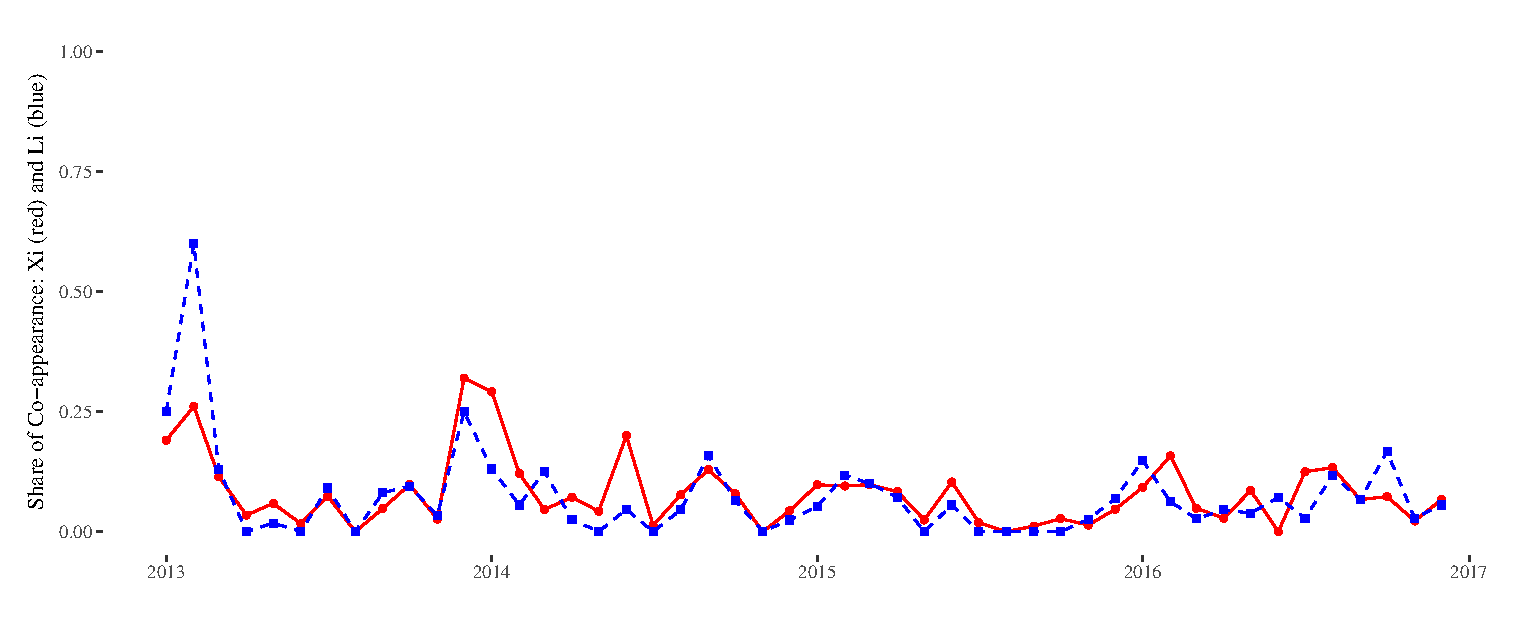
\includegraphics[width=.8\textwidth]{Xi_Li} \\
  \includegraphics[width=.8\textwidth]{Xi_Zg} \\
\end{tabular}
}


\frame{
  \frametitle{Methodology}
\begin{itemize}
\item Use Latent Factor Model (Hoff 2008, Minhas et al 2019, Hoff 2021) to account for 1st/2nd/3rd order dependenices.
\begin{align}
Y & =f(\theta)\\
\theta & =\beta^{\top}\mathbf{X}+Z\\
Z & =M+E\\
M & =U\Lambda U^{\top}
\end{align}
\item Null model, no covariates, no actor random effects, we just want to get out the multiplicative effect to figure out 3rd order dependencies.
\end{itemize}

}
\frame{
  \frametitle{Methodology}
Interpreting the $U\LambdaU^{T}$ matrix
\begin{itemize}
\item U is an $n x k$ matrix that embeds actors in a k dimensional vector space. (k = 2)
\item Actors with vectors pointing in similar directions are likely to share third order ties.
\item For example -- consider an elite and his protege's protege. These actors will often have few coappearances but have very strong 3rd order ties.
\item To measure this similarity we generate a measure of cosine similarity which we term "latent angle distance".
\end{itemize}
}




\frame{
  \frametitle{Latent Positions}

The positions of actors in the $U$ space estimated from the null latent factor model projected onto a unit circle

\centering
\begin{tabular}{lr}
  \includegraphics[width=.45\textwidth]{politSC18_circplot} &  \includegraphics[width=.45\textwidth]{politSC19_circplot} \\
\end{tabular}

}

\frame{
  \frametitle{Downstream Model}
\begin{itemize}
\item Trying to predict appointment to the Leading Small Group.
\item More informal and individual driven policy making committees
\item Two types of LSG: Central Committee and State Council, with appointment controlled by the chairman (Xi) and the premiere (Li Keqiang) respectively
\item We use appointment to the LSG as our DV of a Negative Binomial Model, with the following covariates
\begin{enumerate}
\item Total appearances at events
\item Direct coappearances with Xi Jinping (or Li)
\item Latent angle measure of similarity to Xi (Li)
\end{enumerate}
\end{itemize}
}

\frame{
  \frametitle{Negative binomial regressions on appointment to LSGs}
\resizebox{\textwidth}{!}{%
\centering
\begin{tabular}{ l D{.}{.}{2}D{.}{.}{2}D{.}{.}{2} }
\hline\hline
  & \multicolumn{ 1 }{ c }{ Total Appearances } & \multicolumn{ 1 }{ c }{ Total Appearances } & \multicolumn{ 1 }{ c }{ Total Appearances } \\
  & \multicolumn{ 1 }{ c }{  } & \multicolumn{ 1 }{ c }{ \& Coappearances } & \multicolumn{ 1 }{ c }{ \& Latent Distance } \\ \hline
(Intercept)               & -0.02                     & -0.07                     & -0.23                    \\
                          & (0.16)                    & (0.17)                    & (0.18)                   \\
Total Appearances         & 0.01 ^{***}                & 0.02 ^{*}            & 0.01 ^{**}                  \\
                          & (0.00)                    & (0.01)                    & (0.00)                   \\
% Theta                     & 0.61 ^{***}               & 0.64 ^{***}               & 0.69 ^{***}              \\
%                           & (0.18)                    & (0.19)                    & (0.20)                   \\
Coappearances with Xi     &                           & -0.08                     &                          \\
                          &                           & (0.07)                    &                          \\
Latent Distance from Xi   &                           &                           & -0.80 ^{***}              \\
                          &                           &                           & (0.28)                    \\
%  $N$                       & 111                       & 111                       & 111                      \\
% AIC                       & 335.98                    & 336.57                    & 331.58                   \\
% BIC                       & 368.49                    & 379.92                    & 374.93                   \\
% $\log L$                 & -155.99                   & -152.28                   & -149.79                   \\
\hline\hline
 % \multicolumn{4}{l}{\footnotesize{Standard errors in parentheses}}\\
\textit{Note:} & \multicolumn{3}{r}{\footnotesize{$^*$ significant at $p<.10$; $^{**} p<.05$; $^{***} p<.01$}}
\end{tabular}}

}

\frame{
  \frametitle{Impact of Similarity to Xi}

Substantive effect of our latent distance from Xi variable on predicted number of Leading Small Group (LSG) appointments 

\centering
  \includegraphics[width=\textwidth]{effects.pdf}

}

\frame{
  \frametitle{Out of Sample Model Performance}
  \resizebox{\textwidth}{!}{%
\begin{tabular}{lcccc}
  \\[-1.8ex]\hline
  \hline \\[-1.8ex]
  Model & Logarithmic & Brier & Spherical & RMSE\\    \hline \\[-1.8ex]
Total Appearance & 1.77 & -0.36 & -0.64 & 1.89 \\
Total and Coappearance & 1.77 & -0.38 & -0.66 & 1.84 \\
Total Appearance and  & \multirow{2}{*}{1.73} & \multirow{2}{*}{-0.46} & \multirow{2}{*}{-0.86} & \multirow{2}{*}{1.74} \\
  \;\;\; Latent Distance to Xi &  &  &  &  \\
    \hline
 \hline \\[-1.8ex]
\end{tabular}
}
}

\frame{
  \frametitle{Bivariate probit analyses of CC and SC LSGs}
  \resizebox{\textwidth}{!}{%
  \begin{tabular}{@{\extracolsep{0pt}} l D{.}{.}{2.2} D{.}{.}{2.2} D{.}{.}{2.2} D{.}{.}{2.2}  }
 \\[-1.8ex]\hline
 \hline \\[-1.8ex]
 \\[-1.8ex] & \multicolumn{2}{c}{Latent Distance to Xi} & \multicolumn{2}{c}{Latent Distance to Li}\\
 \\[-1.8ex] & \multicolumn{1}{c}{CC} & \multicolumn{1}{c}{SC} & \multicolumn{1}{c}{CC} & \multicolumn{1}{c}{SC} \\
 \hline
 & & & & \\
 Total appearances     & 0.05^{***} &-0.00     & 0.06^{***} &-0.00 \\
                       &(0.02)      &(0.00)     &(0.02)      &(0.00)\\
 Latent distance to Xi &-0.62^{**}  &-0.26       &            & \\
                       & (0.29)      &(0.23)      &            &\\
 Latent distance to Li &            &            &-0.34       &-1.86^{***}\\
                       &            &            &(0.36)      &(0.40)\\
 % & & & & \\
 % Intercept 1 & \multicolumn{2}{c}{$-1.20^{***}$} & \multicolumn{2}{c}{$-1.19^{***}$}\\
 %             & \multicolumn{2}{c}{(0.19)}        & \multicolumn{2}{c}{(0.21)}\\
 % Intercept 2  & \multicolumn{2}{c}{$-0.70^{***}$} & \multicolumn{2}{c}{$-1.34^{***}$}\\
 %             & \multicolumn{2}{c}{(0.15)}        & \multicolumn{2}{c}{(0.23)}\\
 % Intercept 3 & \multicolumn{2}{c}{$0.93^{**}$}   & \multicolumn{2}{c}{$0.91^{**}$}\\
 %             & \multicolumn{2}{c}{(0.02)}        & \multicolumn{2}{c}{(0.44)}\\
 & & & & \\
 \hline
 \hline \\[-1.8ex]
 \textit{Note:}  & \multicolumn{4}{r}{$^{*}p<$0.1; $^{**}p<$0.05; $^{***}p<$0.01} \\
 \end{tabular}
\
}
}


\frame{
  \frametitle{Conclusion}
  \begin{itemize}
  \item Latent factor approach and public events can give us leverage on opaque, informal behaviour in autocratic states.
  \item Potential new source of data (appearances) for the study of authoritarian politics.
  \item Network based approach trounces dyadic measures on this data.
  \item Measure not only predicts a novel empirical fact (appointment to the LSG) but it discriminates between types of LSGs as institutional power would predict.
  \item Evidence of Xi Jinping's growing informal power between 2013-2017
  \end{itemize}
}
\frame{
  \frametitle{Future Steps}
  \begin{itemize}
  \item Figure out who is important/powerful endogeneously.
  \item Larger timespan and time varying network.
  \item Connect factions/latent connections/LSG membership to policy outcomes.
  \end{itemize}
}

\plain{Thanks for your time! Questions?}

%%%%%%%%%%%%%%%%%%%%%%%%%%%%%%%%%%%%%%%%%%%%%%%%%%%%%%%%%%%%

%%%%%%%%%%%%%%%%%%%%%%%%%%%%%%%%%%%%%%%%%%%%%%%%%%%%%%%%%%%%
%%%%%%%%%%%%%%%%%%%%%%%%%%%%%%%%%%%%%%%%%%%%%%%%%%%%%%%%%%%%

\end{document}
